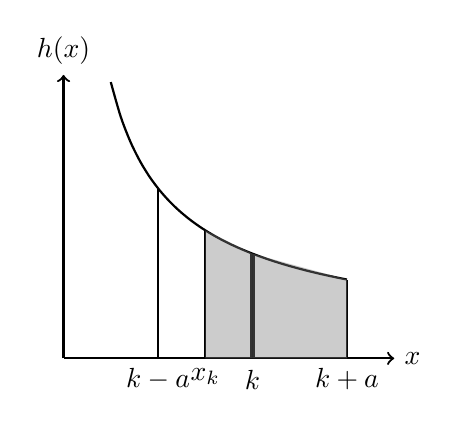
\begin{tikzpicture}[scale=1.2]
    % Axes
    \draw[thick,->] (0,0) -- (3.5,0) node[right] {$x$};
    \draw[thick,->] (0,0) -- (0,3) node[above] {$h(x)$};

    \draw[thick, domain=0.5:3, smooth, variable=\x] plot ({\x}, {1.8/\x^(0.7)});

    % Vertical lines
    \draw[thick] (1,0) node[below] {$k-a$} -- (1,{1.8});
    \draw[thick] (1.5,0) node[below] {$x_k$} -- (1.5,{1.8/(1.5^0.7)});
    \draw[ultra thick] (2,0) node[below] {$k$} -- (2,{1.8/(2^0.7)});
    \draw[thick] (3,0) node[below] {$k+a$} -- (3,{1.8/(3^0.7)});

    % Shaded areas (rejection and acceptance)
    \fill[gray,opacity=0.4] (1.5,0) -- (1.5,{1.8/(1.5^0.7)}) -- (2,{1.8/(2^0.7)}) -- (2,0) -- cycle;
    \fill[gray,opacity=0.4] (2,0) -- (2,{1.8/(2^0.7)}) -- (3,{1.8/(3^0.7)}) -- (3,0) -- cycle;

\end{tikzpicture}
